% ============================================================
% poster.tex — Academic Recruiting Poster
% "Stochastic Attention via Langevin Dynamics on the Modern Hopfield Energy"
% Alswaidan & Varner, Cornell University
%
% Compile with: pdflatex poster.tex
% Figures referenced from ../paper/figs/
% Logo from  logo/cornell_logo.pdf
% ============================================================

\documentclass[final]{beamer}

% --- Poster size: 36" x 48" portrait (91.44 cm x 121.92 cm) ---
\usepackage[orientation=portrait, size=custom,
            width=91.44, height=121.92, scale=1.0]{beamerposter}

\usepackage[utf8]{inputenc}
\usepackage[T1]{fontenc}
\usepackage{lmodern}
\usepackage{graphicx}
\usepackage{booktabs}
\usepackage{amsmath,amssymb}
\usepackage{xcolor}
\usepackage{tikz}
\usepackage{microtype}
\usepackage{array}
\usepackage{ragged2e}
\usepackage{enumitem}

% ============================================================
% Cornell color palette
% ============================================================
\definecolor{CornellRed}{RGB}{179,27,27}
\definecolor{CornellLightGray}{RGB}{247,247,247}
\definecolor{CornellMidGray}{RGB}{200,200,200}
\definecolor{CornellDarkGray}{RGB}{70,70,70}

% ============================================================
% Beamer theme
% ============================================================
\usetheme{default}
\setbeamertemplate{navigation symbols}{}

\setbeamercolor{background canvas}{bg=white}
\setbeamercolor{block title}{fg=white, bg=CornellRed}
\setbeamercolor{block body}{fg=black, bg=CornellLightGray}
\setbeamercolor{block alerted title}{fg=white, bg=CornellDarkGray}
\setbeamercolor{block alerted body}{fg=black, bg=white}

\setbeamerfont{block title}{size=\large, series=\bfseries}
\setbeamerfont{block body}{size=\normalsize}

% Compact block templates
\setbeamertemplate{block begin}{%
  \vskip4pt
  \begin{beamercolorbox}[rounded=true,shadow=false,leftskip=0.8em,
      colsep*=0.5ex]{block title}%
    \usebeamerfont{block title}\insertblocktitle%
  \end{beamercolorbox}%
  \begin{beamercolorbox}[rounded=true,shadow=false,colsep*=0.5ex,vmode,
      leftskip=0.5em,rightskip=0.5em]{block body}%
    \usebeamerfont{block body}\vskip4pt%
}
\setbeamertemplate{block end}{%
  \vskip4pt\end{beamercolorbox}\vskip6pt%
}

\setbeamertemplate{block alerted begin}{%
  \vskip4pt
  \begin{beamercolorbox}[rounded=true,shadow=false,leftskip=0.8em,
      colsep*=0.5ex]{block alerted title}%
    \usebeamerfont{block title}\insertblocktitle%
  \end{beamercolorbox}%
  \begin{beamercolorbox}[rounded=true,shadow=false,colsep*=0.5ex,vmode,
      leftskip=0.5em,rightskip=0.5em]{block alerted body}%
    \usebeamerfont{block body}\vskip4pt%
}
\setbeamertemplate{block alerted end}{%
  \vskip4pt\end{beamercolorbox}\vskip6pt%
}

% ============================================================
\begin{document}
\begin{frame}[t]

% ============================================================
% HEADER: Logo | Title | Authors (left-justified, aligned with logo)
% ============================================================
\vspace*{4pt}
\begin{columns}[c, totalwidth=\linewidth]

  \begin{column}{0.10\linewidth}
    \centering
    
\includegraphics[width=0.88\linewidth]{logo/cornell_logo.pdf}
  \end{column}

  \begin{column}{0.88\linewidth}
    \raggedright
    {\color{black}\bfseries\fontsize{56}{64}\selectfont
      Stochastic Attention via Langevin Dynamics on the Modern Hopfield Energy}\\[8pt]
    {\fontsize{34}{40}\selectfont
      Abdulrahman Alswaidan \& Jeffrey D.\ Varner}\\[6pt]
    {\fontsize{26}{32}\selectfont\color{black}
      R.F.\ Smith School of Chemical and Biomolecular Engineering, Cornell University
      \quad \texttt{\{aa2725, jdv27\}@cornell.edu}}
  \end{column}

\end{columns}

\vspace{16pt}
\textcolor{black}{\rule{\linewidth}{3pt}}
\vspace{2pt}

% ============================================================
% BODY — two equal columns
% ============================================================
\begin{columns}[t, totalwidth=\linewidth]

% ################################################################
% LEFT COLUMN
% ################################################################
\begin{column}{0.475\linewidth}

% -----------------------------------------------------------
\begin{block}{Motivation}
% -----------------------------------------------------------
\justifying
Attention heads are deterministic: the same query always returns the same softmax-weighted memory average.
Yet many tasks require \emph{generating} novel, plausible patterns from structured memory.

We show that the gradient of the \textbf{modern Hopfield energy} is exactly the identity minus the attention map, and that applying \textbf{Langevin dynamics} to this energy yields \emph{stochastic attention}: a \textbf{training-free sampler} controlled by a single inverse temperature $\beta$.

\vspace{4pt}
\begin{center}
\begin{tikzpicture}[font=\small]
  \draw[CornellRed, line width=1.5pt, rounded corners=4pt]
    (0,0) rectangle (0.94\linewidth, 1.2cm);
  \node[anchor=west] at (0.2cm, 0.6cm) {%
    \parbox{0.88\linewidth}{\centering
      $\beta\!\to\!\infty$: exact retrieval \hfill
      $\beta \approx \beta^*$: \textbf{generation of novel patterns} \hfill
      $\beta\!\to\!0$: isotropic noise
    }%
  };
\end{tikzpicture}
\end{center}

\vspace{2pt}
\textbf{No score network, no training loop, no contrastive objective.}
Because the score $\nabla\!\log p_\beta = \beta(\mathbf{T}-\boldsymbol{\xi})$ is the attention map itself, any pretrained attention head becomes a zero-shot stochastic sampler.
\end{block}

% -----------------------------------------------------------
\begin{block}{Method: Stochastic Attention Update}
% -----------------------------------------------------------
\textbf{Setup.}
$\mathbf{X} = [\mathbf{m}_1,\dots,\mathbf{m}_K]\!\in\!\mathbb{R}^{N\times K}$ stores $K$ patterns.
Sample from the Boltzmann distribution $p_\beta(\boldsymbol{\xi})\!\propto\!\exp(-\beta E(\boldsymbol{\xi}))$ using ULA:

\vspace{4pt}
\begin{beamercolorbox}[rounded=true, colsep*=.4ex, leftskip=0.5em, rightskip=0.5em]{block title}
\vspace{2pt}
\[
  \boldsymbol{\xi}_{t+1}
  = \underbrace{(1-\alpha)\,\boldsymbol{\xi}_t}_{\text{contraction}}
  + \underbrace{\alpha\,\mathbf{X}\,\mathrm{softmax}(\beta\,\mathbf{X}^\top\!\boldsymbol{\xi}_t)}_{\text{attention pull to memories}}
  + \underbrace{\sqrt{\tfrac{2\alpha}{\beta}}\;\boldsymbol{\epsilon}_t}_{\text{Gaussian noise}}
\]
\vspace{2pt}
\end{beamercolorbox}

\vspace{6pt}
\begin{itemize}[leftmargin=1.2em, itemsep=1pt]
  \item \textbf{Step cost:} $\mathcal{O}(NK)$ — same as one attention head.
  \item \textbf{No learned parameters.} $\mathbf{X}$ is fixed; no training required.
  \item \textbf{Convergence (convex regime,} $\beta\sigma_{\max}^2 < 2$\textbf{):} $W_2$-geometric convergence; MALA acceptance $= 99.2\%$ at $\alpha\!=\!0.01$ confirms negligible ULA bias.
  \item \textbf{All} $\beta\!>\!0$: the continuous-time SDE is geometrically ergodic (dissipativity of $E$).
\end{itemize}

\vspace{4pt}
\textbf{Temperature selection via entropy inflection.}
The attention entropy $H(\beta)$ transitions from $\log K$ (uniform) to $0$ (hard attention).
Setting $d^2H/d\beta^2\!=\!0$ identifies the retrieval--generation boundary $\beta^*$.
For random unit-norm memories:
\[
  \beta^* \sim \sqrt{N},
  \qquad
  \mathrm{SNR}^* = \sqrt{\tfrac{\alpha\beta^*}{2N}} \sim N^{-1/4}.
\]
For structured data (e.g., protein sequences with conserved residues), evaluate the inflection numerically.
\end{block}

% -----------------------------------------------------------
\begin{block}{Experiment 1 — Phase Behavior \& Convergence (Synthetic)}
% -----------------------------------------------------------
\begin{center}
  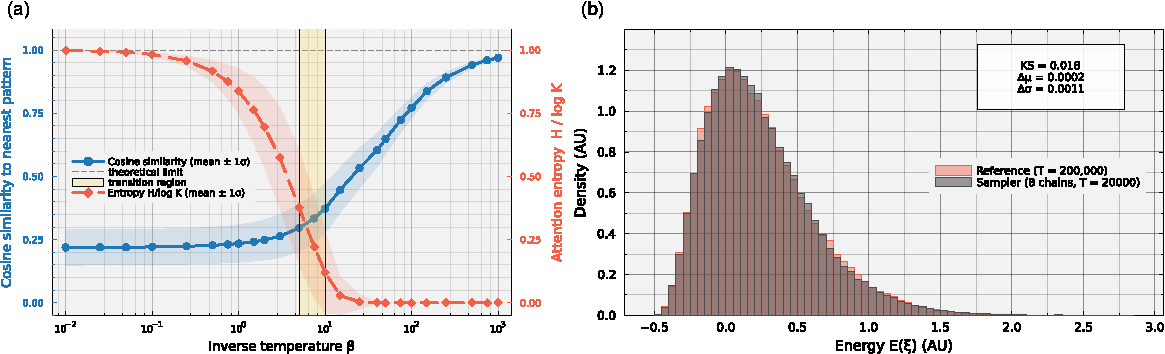
\includegraphics[width=0.96\linewidth]{../paper/figs/Fig_experiment-combined.pdf}
\end{center}
{\small
\textbf{(a)} $d\!=\!64$, $K\!=\!16$.
Cosine similarity (blue) and scaled entropy (coral) exhibit a smooth sigmoidal transition centered at $\beta\!\approx\!5$--$10$ (gold band), consistent with the predicted $\beta^*\!\sim\!\sqrt{N}$.\\[2pt]
\textbf{(b)} $d\!=\!8$, $K\!=\!4$, $\beta\!=\!5$.
Eight independent chains (gray) converge to a long-run reference (coral); KS statistic confirms the correct Boltzmann target.
}
\end{block}

\end{column}
% end LEFT COLUMN

% ################################################################
% RIGHT COLUMN
% ################################################################
\begin{column}{0.475\linewidth}

% -----------------------------------------------------------
\begin{block}{Experiment 2 — Load Ratio Phase Diagram (Synthetic)}
% -----------------------------------------------------------
\begin{center}
  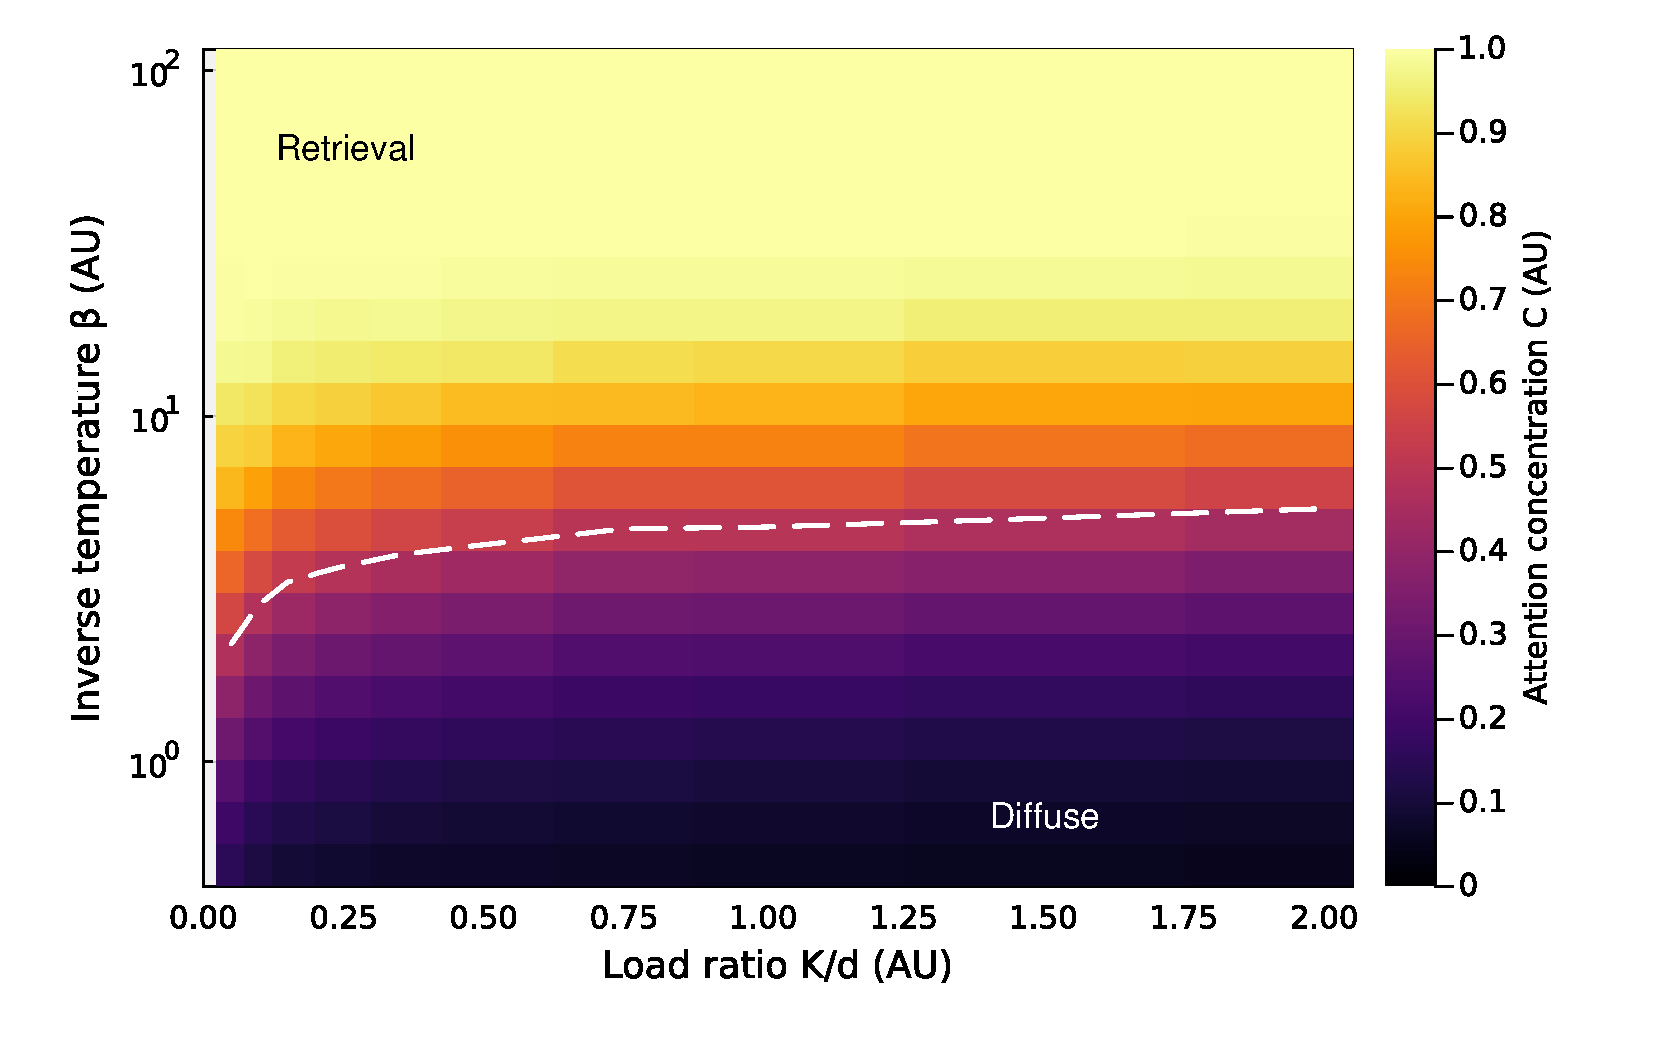
\includegraphics[width=0.80\linewidth]{../paper/figs/Fig_experiment-3-load-ratio.pdf}
\end{center}
{\small
Attention concentration $C\!=\!1\!-\!H(\mathbf{a})/\log K$ over load ratio $K/d$ and $\beta$ ($d\!=\!64$).
The $C\!=\!0.5$ phase boundary (dashed) shifts right with increasing $\beta$: higher temperature extends reliable retrieval to larger memory loads, consistent with classical Hopfield capacity theory.
}
\end{block}

% -----------------------------------------------------------
\begin{block}{Experiment 3 — MNIST Image Generation ($K=100$, $d=784$)}
% -----------------------------------------------------------
\textbf{Setup.} 100 images of digit ``3''; 30 independent chains; 150 generated samples.
$\beta\!=\!2000$ (SNR$\!=\!0.113$, retrieval) and $\beta\!=\!200$ (SNR$\!=\!0.036$, generation).

\vspace{4pt}
\begin{center}
{\small
\setlength{\tabcolsep}{5pt}
\begin{tabular}{@{}lccc@{}}
\toprule
\textbf{Method} & \textbf{Novelty}$\uparrow$ & \textbf{Diversity}$\uparrow$ & \textbf{Energy}$\downarrow$ \\
\midrule
Bootstrap            & $0.000$ & $0.459$ & $-0.500$ \\
Gaussian perturbation & $0.004$ & $0.450$ & $-0.496$ \\
Random convex combo  & $0.092$ & $0.008$ & $-0.399$ \\
GMM-PCA              & $0.198$ & $0.419$ & $-0.303$ \\
VAE (latent $=8$)    & $0.214$ & $0.441$ & $-0.286$ \\
DDPM\textsuperscript{\dag} & $0.938$ & $0.991$ & $+0.44$ \\
MALA ($\beta\!=\!2000$)   & $0.151$ & $0.598$ & $-0.305$ \\
SA ($\beta\!=\!2000$, retrieval) & $0.152$ & $0.600$ & $-0.303$ \\
\textbf{SA ($\beta\!=\!200$, generation)} & $\mathbf{0.548}$ & $\mathbf{0.885}$ & --- \\
\bottomrule
\end{tabular}
}
\end{center}

\vspace{2pt}
{\small\textsuperscript{\dag}DDPM produces isotropic noise (max-cos $=0.062$) despite 5,000 training epochs.}

\vspace{4pt}
SA at $\beta\!=\!200$ achieves $\mathbf{2.6\times}$ the novelty and $\mathbf{2.0\times}$ the diversity of the best learned baseline (VAE), while matching the Metropolis-corrected MALA gold standard.
\end{block}

% -----------------------------------------------------------
\begin{block}{Experiment 4 — Protein Sequence Generation (Pfam RRM, $K=68$, $d=59$)}
% -----------------------------------------------------------
\textbf{Setup.} 68 aligned RRM sequences; one-hot encoded, PCA-reduced (95\% variance).
Entropy inflection gives $\beta^*\!=\!3.85$ (half the random-pattern prediction $\sqrt{d}\!=\!7.68$; conserved residues increase effective similarity variance).

\vspace{4pt}
\begin{center}
{\small
\setlength{\tabcolsep}{5pt}
\begin{tabular}{@{}lcccc@{}}
\toprule
\textbf{Method} & \textbf{Novelty}$\uparrow$ & \textbf{Diversity}$\uparrow$ & \textbf{SeqID} & \textbf{KL}$\downarrow$ \\
\midrule
Bootstrap          & $0.000$ & $1.000$ & $0.645$ & $0.133$ \\
VAE (latent $=8$)  & $0.621$ & $0.834$ & $0.532$ & $0.416$ \\
SA ($\beta\!=\!77$, retrieval)  & $0.243$ & $0.991$ & $0.616$ & $0.107$ \\
\textbf{SA ($\beta\!=\!8$, generation)} & $\mathbf{0.623}$ & $\mathbf{1.001}$ & $0.538$ & $\mathbf{0.060}$ \\
\bottomrule
\end{tabular}
}
\end{center}

\vspace{4pt}
SA matches the VAE on novelty while achieving $\mathbf{6.9\times}$ lower amino acid composition divergence (KL $= 0.060$ vs.\ $0.416$).
The training-free Langevin score preserves family-level fidelity that learned models cannot maintain at small $K$.
\end{block}

% -----------------------------------------------------------
\begin{alertblock}{Limitations \& Future Work}
% -----------------------------------------------------------
\begin{itemize}[leftmargin=1.2em, itemsep=2pt]
  \item \textbf{ULA bias} scales with step size $\alpha$; MALA (with Metropolis correction) is preferred at larger $\alpha$.
  \item \textbf{Inter-basin mixing} at high $\beta$ is exponentially slow; the multi-chain protocol provides a practical workaround, but quantitative scaling laws remain open.
  \item \textbf{Fixed memory:} $\mathbf{X}$ must be known at sampling time; streaming or latent memory settings require extension.
  \item \textbf{Generation fidelity} at high temperature yields structured interpolations rather than crisp samples; operating near $\beta^*$ improves quality.
  \item \textbf{Future:} multi-head attention, hierarchical memories, retrieval-augmented generation, in-context learning.
\end{itemize}
\end{alertblock}

\end{column}
% end RIGHT COLUMN

\end{columns}

% ============================================================
% FOOTER
% ============================================================
\vfill
\textcolor{CornellMidGray}{\rule{\linewidth}{2pt}}
\vspace{2pt}
\begin{columns}[c, totalwidth=\linewidth]
  \begin{column}{0.55\linewidth}
    {\footnotesize\color{CornellDarkGray}
      This work grew out of CHEME-5820: Machine Learning \& AI Methods for Engineers, Cornell University.
    }
  \end{column}
  \begin{column}{0.44\linewidth}
    \raggedleft
    {\footnotesize\color{CornellDarkGray}
      \texttt{github.com/varnerlab/stochastic-attention-study-paper}
    }
  \end{column}
\end{columns}

\end{frame}
\end{document}
